\mode<presentation>
{
  \usetheme{CambridgeUS}
  \usecolortheme{whale}
  \usecolortheme{lily}

  \setbeamercovered{transparent}
  \usefonttheme[onlymath]{serif}
}

\title[\FluidandAnalogousSystemsShortName] 
{\course: \FluidandAnalogousSystemsName\license}

\subtitle{Lecture \FluidandAnalogousSystemsNumber}



\begin{document}

\begin{frame}
  \titlepage
\end{frame}

\mode<article>{
\maketitle
\tableofcontents
}

%\mode<presentation>{
%\begin{frame}{Outline}
%  \tableofcontents
%  % You might wish to add the option [pausesections]
%\end{frame}}

\section{Pre-requisite Material}
This lecture assumes that the reader is familiar with the following material:
\begin{itemize}
\item Lecture \ImpedanceNumber:~\ImpedanceName
\end{itemize}



\section{Incompressible Fluid Systems}
For fluid systems, the variables that we are modeling are 
\begin{itemize}
\item Pressure, which has units of Newtons per meter squared [Nm$^{-2}$] or equivalently [kg m$^{-1}$s$^{-2}$]
\item Volumetric Flow, which has units of meters cubed per second [m$^{3}$s$^{-1}$]. 
\end{itemize}

\subsection{Components}

\begin{frame}{Tank}
The change in the volume of fluid inside the tank is equal to the difference between the input and output volumetric flow. 
\begin{center}
\input{figures/tank.tex}
\end{center}
\end{frame}
If $V$ is the volume of fluid, then the change in the amount of fluid in the tank over time is equal to the volumetric flow in minus the volumetric flow out, so that 
\begin{equation}\label{eqn:flow1}
\frac{dV}{dt} = q_{1}-q_{2}.
\end{equation}
For a tank with constant cross-sectional area $A$ m$^2$, $V=Ah$, so taking the derivative of both sides with respect to time gives us 
\begin{equation}\label{eqn:flow2}
\frac{dV}{dt}=A\frac{dh}{dt}.
\end{equation}
Setting (\ref{eqn:flow1}) equal to (\ref{eqn:flow2}) gives us the equation
\[
A\frac{dh}{dt} = q_{1} - q_{2}.
\]
This can also be written in terms of the pressure difference between the bottom and top of the tank, since $p_{1}-p_{2} = \rho g h$, where $\rho$ is the fluid density [kg m$^{-3}$], and $g$ is gravitational acceleration [m s$^{-2}$]. Substituting for $h$ results in
\[
\frac{A}{\rho g}\frac{d(p_{1}-p_{2})}{dt} = q_{1} - q_{2}.
\]


\begin{frame}{Linear Valve}
A valve causes a restriction that causes the pressure on one end of the value to be higher than the other end. When this pressure drop is proportional to the flow, the valve is linear with valve constant $R$. (Most valves are nonlinear, however.) By unit analysis, the units of valve resistance are [N s m$^{-5}$] or equivalently [kg m$^{-4}$s$^{-1}$].
\begin{center}
\input{figures/valve.tex}
\end{center}
\end{frame}

Why only two elements? We have not considered fluid inertia.

\subsection{Connection Rules and Boundary Conditions}

The connection rules and boundary conditions will sound familiar
\begin{itemize}
\item When elements are connected, the two components share the same {\em pressure}. 
\item When elements are connected, the {\em flows} sum to zero. 
\item Boundary conditions can set either the pressure or flow of one side of a component
\end{itemize}

\subsection{Example}
Find the differential  equation that describes the relationship between $q_{in}$, and $h$ for the following system:
\begin{frame}{Tank and Valve Example}
Assume the valve is linear with valve constant $R$ and that the density of the fluid is $\rho$. The valve empties to atmospheric pressure, $p_{a}$, which is the same as the pressure at the top of the tank.
\begin{center}
\begin{tikzpicture}
\draw (.75,0) node[above] (tank) {\input{\mainfolder/DrawingElements/FluidElements/tank.tex}};
\draw[decorate,decoration={coil,aspect=0,segment length=5.85pt}] (-.45,2.25) -- ++(2.38,0);
\draw (-1.15,1) node (pipe1) {\input{\mainfolder/DrawingElements/FluidElements/pipe.tex}};
\draw (2.65,1) node (pipe2) {\input{\mainfolder/DrawingElements/FluidElements/valve.tex}};
\draw[->] (.2,.75) -- node[pos=.5,left] {$h$} ++(0,1.4);
\draw (tank.-90) node{Tank Area: $A$};
\draw (pipe2.90) node[above] {$R$};
\draw (.75,.8) node[above] {$p_{1}$};
\draw[<-] (pipe1.180) ++(.5,0) --  ++(-.5,0) node[left] {$q_{in}$};
\draw[->] (pipe2.0) ++(-.5,0) --  ++(.5,0) node[right] {$q_{out}$};
\draw (.75,2.5) node[above] {$p_{a}$};
\draw (pipe2.0) ++(1.5,0) node {$p_{a}$};
\end{tikzpicture}
\end{center}
\end{frame}

We use the following steps:
\begin{itemize}
\item Write down the component laws for the tank and valve, along with connection laws where applicable.
\item Write down the relationship between the pressures and the tank height.
\item Eliminate unwanted variables. 
\end{itemize}
The component laws are:
\begin{align*}
A\frac{dh}{dt} &= q_{in} - q_{out}, \\
p_{1} - p_{2} &= Rq_{out}.
\end{align*}
Note that we used a connection law to establish that the flow out of the tank is $q_{out}$, the pressure at the left side of the valve is $p_{1}$, and the pressure on the right side of the valve is $p_{a}$ where $p_a$ corresponds to $p_2$ in the component law above.  We also know that
\[
\rho g h = p_{1} - p_{2}.
\] 
Thus,
\begin{align*}
A\frac{dh}{dt} &= q_{in} - q_{out}, \\
\rho g h &= Rq_{out}.
\end{align*}
Eliminating $q_{out}$,
\[
A\frac{dh}{dt} = q_{in} - \frac{\rho g}{R} h, \\
\]
or
\[
A \frac{dh}{dt} + \frac{\rho g}{R} h = q_{in}.  \\
\]
\section{System Analogies}
Thus far, we have modeled translational mechanical systems, electrical systems, and fluid systems using lumped, linear elements. We have seen a lot of commonalities:
\begin{itemize}
\item Two variables are important.
\item Each element relates these two variables via a linear algebraic or differential relationship.
\item There are two connection rules that govern how the two variables are related at a connection point.
\end{itemize}
We can use these commonalities to come up with a modeling method that could applied to all of the domains we have discussed so far. 

\subsection{Generic Modeling Elements}
Physical system modeling requires us to keep track of two variables. The one that is measured on each side of an element is called the {\em across} variable, and the one whose magnitude is the same on each side is the {\em through} variable. The component law is a linear algebraic or differential relationship between these two variables.
\begin{frame}{Generic Lumped Element}
\begin{center}
\input{figures/genericelement.tex}
\end{center}
\end{frame}

When the components are connected, we apply generic connection rules to the across and through variables.
\begin{frame}{Generic Connection Rules}
\begin{center}
\begin{tikzpicture}
\draw (-1,0) node[rectangle,draw,minimum width=.5in,minimum height=.1in] (e) {};
\draw (-1,0) node[above=9pt] {$R_{1}$};
\draw (1,0) node[rectangle,draw,minimum width=.5in,minimum height=.1in] (f) {};
\draw (1,0) node[above=9pt] {$R_{2}$};
\draw[very thick] (-2.25,0) -- (e.180);
\draw[very thick] (e.0) -- (f.180);
\draw[very thick] (f.0) -- (2.25,0);

\draw (-2,-2) node {\begin{tikzpicture}
\draw (.75,0) node[rectangle,draw,minimum width=.5in,minimum height=.1in] (e) {};
\draw[very thick] (-.5,0) -- (e.180);
\draw[very thick] (e.0) -- (2,0);
\draw (.75,0) node[above=9pt] {$R$};
\draw (-.2,.25) node[above] {$\alpha_{1}$};
\draw[<-] (-.52,0) -- node[below] {$\eta_{1}$} ++(-.5,0);
\draw[->] (2.02,0) -- node[below] {$\eta_{1}$} ++(.48,0);
\draw (1.7,.25) node[above] {$\alpha_{2}$};
\end{tikzpicture}};

\draw (2,-2) node {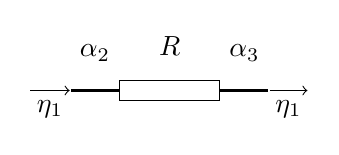
\begin{tikzpicture}
\draw (.75,0) node[rectangle,draw,minimum width=.5in,minimum height=.1in] (e) {};
\draw[very thick] (-.5,0) -- (e.180);
\draw[very thick] (e.0) -- (2,0);
\draw (.75,0) node[above=9pt] {$R$};
\draw (-.2,.25) node[above] {$\alpha_{2}$};
\draw[<-] (-.52,0) -- node[below] {$\eta_{1}$} ++(-.5,0);
\draw[->] (2.02,0) -- node[below] {$\eta_{1}$} ++(.48,0);
\draw (1.7,.25) node[above] {$\alpha_{3}$};
\end{tikzpicture}};
\end{tikzpicture}
\end{center}
\end{frame}
\begin{itemize}
\item When elements are connected, the two components share the same {\em across variable}. 
\item When elements are connected, the {\em through variables} sum to zero. 
\item Boundary conditions can set either the across or through variables on one side of a component
\end{itemize}

The following table lists the across and through variables for the modeling domains that we will discuss in this course.
\begin{frame}{Across and through variables}
\begin{center}
\begin{tabular}{c|c|c}
Domain & Across Variable & Through Variable \\\hline\hline
Electrical & Voltage & Current \\\hline
Translational Mechanical & Position & Force \\\hline
Fluid & Pressure & Flow \\\hline
Rotational Mechanical & Angular Position & Torque \\\hline
Thermal & Temperature & Heat Flow \\\hline
\end{tabular}
\end{center}
\end{frame}

\begin{remark}
One detail that may seem odd when considering force as a flow variable is the fact that force is defined as acting in opposite directions on the ends of each element. However, despite this, the interconnection rules are exactly the same. That is, for the example below, if the spring and damper are interconnected, we have $f_{k}=f_{b}$, while if the capacitor and inductor are connected, $i_{C}=i_{R}$. So in both cases, the flow variable on the left hand side of one element ``flows'' to the left hand side of the other element.
\end{remark}

\begin{frame}{Force flow vs Current flow}
\begin{center}
\input{figures/springvsresistorflow.tex}
\end{center}

\end{frame}

By utilizing variables that have the same function in different domains, we can come up with system analogies. Analogous systems are systems in different domains that have the same equations describing their behavior.


\begin{frame}{Electrical Analogy for Fluid Elements:}{Tank}
\begin{center}
\begin{tikzpicture}
\draw (.75,0) node[above] {\input{\mainfolder/DrawingElements/FluidElements/tank.tex}};
\draw[decorate,decoration={coil,aspect=0,segment length=5.85pt}] (-.45,2.25) -- ++(2.38,0);
\draw (-1.15,1) node (pipe1) {\input{\mainfolder/DrawingElements/FluidElements/pipe.tex}};
\draw (2.65,1) node (pipe2) {\input{\mainfolder/DrawingElements/FluidElements/pipe.tex}};
\draw[->] (.2,.75) -- node[pos=.5,left] {$h$} ++(0,1.4);
\draw (.75,.65) node[below=9pt] {Tank Area: $A$};
\draw (.75,.8) node[above] {$p_{1}$};
\draw[<-] (pipe1.180) ++(.5,0) --  ++(-.5,0) node[left] {$q_{1}$};
\draw[->] (pipe2.0) ++(-.5,0) --  ++(.5,0) node[right] {$q_{2}$};
\draw (.75,2.5) node[above] {$p_{2}$};
%\draw (-1.25,-.75) node {$A\frac{dH}{dt} = Q_{1} - Q_{2}$};
%\draw (4,2) node{$P_{1}-P_{2} = \rho g H$};
\draw (.75,-.75) node {$\frac{A}{\rho g}\frac{d(p_{1}-p_{2})}{dt} = q_{1} - q_{2}$};


\draw (5.5,3.5) node[inner sep=0,outer sep=0] (a)  {};
\draw (5.5,0.5) node[inner sep=0,outer sep=0] (b) {};
\draw (8.5,3.5) node[inner sep=0,outer sep=0] (c) {};
\draw (8.5,0.5) node[inner sep=0,outer sep=0] (d) {};
\draw (7,3.5) node[circle,draw,fill=black,inner sep=1pt] {} node[above] {$p_{1}$};
\draw (7,0.5) node[circle,draw,fill=black,inner sep=1pt] {} node[below] {$p_{2}$};
\draw (7,2) node[rotate=90,inner sep=0pt,outer sep=0pt] (C) {\input{\mainfolder/DrawingElements/CircuitElements/capacitor.tex}};
\draw (C) node[right=18pt] {$C=\frac{A}{\rho g}$};
\draw[very thick] (a) -| (C.0);
\draw[very thick] (C.0) |- (c);
\draw[very thick] (b) -| (C.180);
\draw[very thick] (C.180) |- (d);
\draw[<-] (a) -- ++(-.5,0) node[left] {$q_{1}$};
\draw[->] (c) -- ++(.5,0) node[right] {$q_{2}$};
\draw (7,-.75) node {$C\frac{d(p_{1}-p_{2})}{dt} = q_{1} - q_{2}$};

\end{tikzpicture}

\end{center}
\end{frame}

\begin{frame}{Electrical Analogy for Fluid Elements:}{Valve}
\begin{center}
\begin{tikzpicture}
\draw (.75,0) node (valve) {\input{\mainfolder/DrawingElements/FluidElements/valve.tex}};
\draw (.75,0) node[above=9pt] {$R$};
\draw (-.2,.25) node[above] {$p_{1}$};
\draw[<-] (valve.180) --  ++(-.5,0) node[left] {$q$};
\draw[->] (valve.0) -- ++(.5,0)  node[right] {$q$};
\draw (1.7,.25) node[above] {$p_{2}$};
\draw (.75,-1) node {$p_{1}-p_{2} = Rq$};

\draw (7,0) node (R) {\input{\mainfolder/DrawingElements/CircuitElements/resistor.tex}};
\draw (R) node[above=9pt] {$R$};
\draw (6.05,.25) node[above] {$p_{1}$};
\draw[<-] (R.180) --  ++(-.5,0) node[left] {$q$};
\draw[->] (R.0) -- ++(.5,0)  node[right] {$q$};
\draw (7.95,.25) node[above] {$p_{2}$};
\draw (7,-1) node {$p_{1}-p_{2} = Rq$};

\end{tikzpicture}
\end{center}
\end{frame}

\section{Fluid Impedances}

With analogies to electrical components, it is very clear what the impedance of fluid components are when we want to use impedance methods to find transfer functions.

For fluid systems, we have the following impedances
\begin{frame}{Fluid Impedances}
\begin{center}
\mode<article>{\begin{tabular}{c|cc}
 & valve & tank \\\hline
Component &\begin{tikzpicture}
\draw (.75,0) node (valve) {\input{\mainfolder/DrawingElements/FluidElements/valve.tex}};
\draw (.75,0) node[above=9pt] {$R$};
\draw (-.2,.25) node[above] {$p_{1}$};
\draw[<-] (valve.180) --  ++(-.5,0) node[left] {$q$};
\draw[->] (valve.0) -- ++(.5,0)  node[right] {$q$};
\draw (1.7,.25) node[above] {$p_{2}$};
\draw (.75,1.5) node {$p = p_{1}-p_{2}$};
\end{tikzpicture} & \input{figures/tank2.tex} \\\hline
\rule[-8pt]{0pt}{0pt}\rule{0pt}{14pt} Component law & $p=Rq$ & $\frac{A}{\rho g}\frac{dp}{dt} = q_{in} - q_{out}$ \\\hline
\rule[-8pt]{0pt}{0pt}\rule{0pt}{14pt} Laplace Transform & $P(s)= RQ(s)$ & $\frac{A}{\rho g}sP(s) = Q_{in}(s)-Q_{out}(s)$ \\\hline
 Impedance Component & \input{figures/valveanalogycopy.tex} & \input{figures/tankanalogycopy.tex}
 \end{tabular}}
\mode<presentation>{\resizebox{11cm}{!}{
\begin{tabular}{c|cc}
 & valve & tank \\\hline
Component &\begin{tikzpicture}
\draw (.75,0) node (valve) {\input{\mainfolder/DrawingElements/FluidElements/valve.tex}};
\draw (.75,0) node[above=9pt] {$R$};
\draw (-.2,.25) node[above] {$p_{1}$};
\draw[<-] (valve.180) --  ++(-.5,0) node[left] {$q$};
\draw[->] (valve.0) -- ++(.5,0)  node[right] {$q$};
\draw (1.7,.25) node[above] {$p_{2}$};
\draw (.75,1.5) node {$p = p_{1}-p_{2}$};
\end{tikzpicture} & \input{figures/tank2.tex} \\\hline
\rule[-8pt]{0pt}{0pt}\rule{0pt}{14pt} Component law & $p=Rq$ & $\frac{A}{\rho g}\frac{dp}{dt} = q_{in} - q_{out}$ \\\hline
\rule[-8pt]{0pt}{0pt}\rule{0pt}{14pt} Laplace Transform & $P(s)= RQ(s)$ & $\frac{A}{\rho g}sP(s) = Q_{in}(s)-Q_{out}(s)$ \\\hline
 Impedance Component & \input{figures/valveanalogycopy.tex} & \input{figures/tankanalogycopy.tex}
 \end{tabular}}}
\end{center}
\end{frame}

Let's return to the earlier tank and valve system and go through the modeling process with analogous elements. 

\begin{frame}{Tank and Valve Problem}

\textit{Example:} Find the equivalent impedance model of the tank and valve system below with input flow $q_{in}$ and output flow $q_{out}$.

\begin{center}
\begin{tikzpicture}
\draw (.75,0) node[above] (tank) {\input{\mainfolder/DrawingElements/FluidElements/tank.tex}};
\draw[decorate,decoration={coil,aspect=0,segment length=5.85pt}] (-.45,2.25) -- ++(2.38,0);
\draw (-1.15,1) node (pipe1) {\input{\mainfolder/DrawingElements/FluidElements/pipe.tex}};
\draw (2.65,1) node (pipe2) {\input{\mainfolder/DrawingElements/FluidElements/valve.tex}};
\draw[->] (.2,.75) -- node[pos=.5,left] {$h$} ++(0,1.4);
\draw (tank.-90) node{Tank Area: $A$};
\draw (pipe2.90) node[above] {$R$};
\draw (.75,.8) node[above] {$p_{1}$};
\draw[<-] (pipe1.180) ++(.5,0) --  ++(-.5,0) node[left] {$q_{in}$};
\draw[->] (pipe2.0) ++(-.5,0) --  ++(.5,0) node[right] {$q_{out}$};
\draw (.75,2.5) node[above] {$p_{a}$};
\draw (pipe2.0) ++(1.5,0) node {$p_{a}$};
\end{tikzpicture}
\end{center}
\end{frame}

\begin{itemize}
\item[Step 1] \textbf{Identify all node variables.} For a fluid problem, the node variables are pressure. There are two unique pressure variables: $p_{1}$, the pressure at the bottom of the tank, and $p_{a}$ atmospheric pressure. Our circuit should thus have two identifiable voltage nodes.

\begin{frame}{Tank system nodes}
\begin{center}
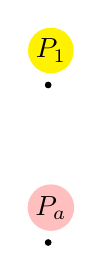
\begin{tikzpicture}
\draw (0,0) node[draw,fill,inner sep=0pt,outer sep=0pt,circle] (T1) {$\rule{2pt}{0pt}$};
\draw (T1.0) node[above=4pt,circle, inner sep=1pt,fill=yellow] {$P_{1}$};
\draw (0,-2) node[draw,fill,inner sep=0pt,outer sep=0pt,circle] (Gnd) {$\rule{2pt}{0pt}$};
\draw (Gnd.0) node[above=4pt,circle, inner sep=1pt,fill=pink] {$P_{a}$};

\end{tikzpicture}
\end{center}
\end{frame}

\item[Step 2] \textbf{Identify one node as ground, or add a ground node.} Most node variables are relative - for example, consider the ground on a circuit diagram. All voltages are measured with respect to ground, so the ground voltage is simply what we will consider to be 0 V. Negative voltages are lower than ground, positive voltages are higher than ground. If we identify a node as the ground, then we will measure all node variables relative to this node. For fluid systems, there are two typical choices: Either choose absolute zero pressure (i.e. a vacuum) as ground, or choose atmospheric pressure as ground. Pressure measured with respect to atmospheric pressure is called {\em gauge} pressure, and the translation is 
\[
\mbox{Absolute Pressure} = \mbox{Gauge Pressure} + \mbox{Atmospheric Pressure}
\]
For this problem, we will choose to measure pressure using gauge pressure, so that node $p_{a}$ will be considered ground.

\item[Step 3] \textbf{Connect components between nodes.} Since flow is a through variable, setting the input flow is done with a current source. The flow is into the node representing pressure $p_{1}$, and all sources representing boundary conditions have the other end connected to ground. We also connect a tank (capacitance) impedance between $p_{1}$ and $p_{a}$, because the pressure at the top of the tank is $p_{a}$. A valve (resistance) impedance is connected between $p_{1}$ and $p_{a}$ because the valve transmits flow from a node at pressure $p_{1}$ to a node at pressure $p_{a}$.

\begin{frame}{Tank system impedance model}
\begin{center}
\begin{tikzpicture}
\draw (-2,-1.5) node[scale=.85,inner sep=0pt,outer sep=0pt] (a) {\input{\mainfolder/DrawingElements/CircuitElements/currentsource.tex}};
\draw (-.5,0) node[circle,fill=black,inner sep=0,minimum width=4pt] {} node[above=4pt,circle, inner sep=1pt,fill=yellow] {$P_{1}$};
\draw (a) node[left=9pt] {$Q_{in}(s)$};
\draw (-.5,-1.5) node[rectangle,draw,minimum width=.1in,minimum height=.5in] (tank1) {};
\draw (tank1) node[right=9pt] {$\frac{\rho g}{sA_{1}}$};
\draw (1,0) node[rectangle,draw,minimum width=.5in,minimum height=.1in] (valve1) {};
\draw (valve1) node[above=9pt] {$R_{1}$};
\draw (2.5,-3) node[inner sep=0] (pa) {};
\draw (-.5,-3) node[circle,fill=black,minimum width=4pt,inner sep=0] {};
\draw (-.5,-3) node[below=4pt,circle, inner sep=1pt,fill=pink] {$P_{a}$};
\draw (2.5,-3) node[inner sep=0,outer sep=0] (pa2) {};
\draw (-.5,-3) node[inner sep=0,outer sep=0] (pa3) {};
\draw[very thick] (a.90) |- (valve1.180);
\draw[very thick] (tank1.90) |- (valve1.180);
\draw[very thick] (valve1.0) -| (pa) -- (pa3);
\draw[very thick] (tank1.-90) -- (pa3) -| (a.-90);
\draw[->] (3,-1) -- node[pos=.5,right] {$Q_{out}(s)$} ++(0,-1);
\end{tikzpicture}
\end{center}
\end{frame}

\end{itemize}



You can now use your circuit simplifications to find any transfer function of interest.


%The resulting analogous system is as follows.
%
%\begin{frame}{Example Analogy}
%\begin{center}
%\resizebox{10cm}{!}{\begin{tikzpicture}[nosep/.style={inner sep=0pt, outer sep=0pt}]
\draw (.75,0) node[above] (tank) {\input{\mainfolder/DrawingElements/FluidElements/tank.tex}};
\draw[decorate,decoration={coil,aspect=0,segment length=5.85pt}] (-.45,2.25) -- ++(2.38,0);
\draw (-1.15,1) node (pipe1) {\input{\mainfolder/DrawingElements/FluidElements/pipe.tex}};
\draw (2.65,1) node (pipe2) {\input{\mainfolder/DrawingElements/FluidElements/valve.tex}};
\draw[->] (.2,.75) -- node[pos=.5,left] {$h$} ++(0,1.4);
\draw (tank.-90) node{Tank Area: $A$};
\draw (pipe2.90) node[above] {$R$};
\draw (.75,.8) node[above] {$p_{1}$};
\draw[<-] (pipe1.180) ++(.5,0) --  ++(-.5,0) node[left] {$q_{in}$};
\draw[->] (pipe2.0) ++(-.5,0) --  ++(.5,0) node[right] {$q_{out}$};
\draw (.75,2.5) node[above] {$p_{a}$};

\draw (6,2) node[nosep,scale=.95] (I) {\input{\mainfolder/DrawingElements/CircuitElements/currentsource.tex}};
\draw (6,2) node[left=18pt] {$q_{in}$};
\draw (8,2) node[rotate=90,nosep] (C) {\input{\mainfolder/DrawingElements/CircuitElements/capacitor.tex}}; 
\draw (8,2) node[right=18pt] {$\frac{A}{\rho g}$};
\draw (9.5,3.5) node[nosep] (R) {\input{\mainfolder/DrawingElements/CircuitElements/resistor.tex}}; 
\draw (9.5,3.5) node[above=12pt] {$R$};
\draw (8,3.5) node[draw,fill=black,circle,inner sep=2pt,outer sep=0pt] (P1) {} node[above] {$p_{1}$};
\draw (8,.5) node[draw,fill=black,circle,inner sep=2pt,outer sep=0pt] (Pa) {} node[below=2pt] {$p_{a}$};
\draw[->] (11,2) ++(.1,.5) -- node[pos=.5,right] {$q_{out}$} ++(0,-1) ;
\draw[very thick] (I.90) |- (R.180);
\draw[very thick] (C.0) |- (P1);
\draw[very thick] (R.0) |- (Pa);
\draw[very thick] (C.180) |- (Pa);
\draw[very thick] (Pa) -| (I.-90);
\end{tikzpicture}}
%\end{center}
%\end{frame}

Again, it should be emphasized that in this case we have chosen the ambient pressure $p_{a}$ as the reference pressure. This means that all pressure nodes in this ``circuit'' are measured with respect to ambient pressure, so that the pressure at node $p_{1}$ is in fact $p_{1}+p_{a}$.

\section{Application Example}
\textit{A real world example information related to a fluid system that must be carefully controlled}\\

\noindent A video explaining what went wrong at the Fukushima Nuclear Reactor in 2011 is available at \url{https://www.youtube.com/watch?v=BdbitRlbLDc}

These two snapshots are from the video and show (top) one of the safety feedback loops and (bottom) the water level dropping in the reactor rod cooling system.

\begin{center}
	\includegraphics[width=5in]{figures/fukushima1.png}
\end{center}
\begin{center}
	\includegraphics[width=5in]{figures/fukushima2.png}
\end{center}

\noindent What do we need to know before we can begin to design the three separate water-cooling-based safety control loops for the nuclear reactor cooling system?\\

\noindent Compare the tank example in Lecture \FluidandAnalogousSystemsNumber
\begin{center}
	\includegraphics[width=3.5in]{figures/fukushimaDiagram1.png}
	\includegraphics[width=1.5in]{figures/fukushimaDiagram2.png}
\end{center}
to the Fukushima set-up
\begin{center}
	\includegraphics[width=3in]{figures/fukushima3.png}
\end{center}

\noindent What are some key simplifications?

% Note: this application example needs a good modeling question associated with it


\section{Lecture Highlights}
The primary takeaways from this article include
\begin{enumerate}
\setlength{\itemsep}{5pt}
\setlength{\parskip}{0pt}
\setlength{\parsep}{0pt}
\item In this class, we model fluid systems using two ideal components: tanks and linear valves.
\item The component law for a tank is a differential equation and the component law for a linear valve is an algebraic equation. You can take the Laplace transform of each equation to find the component's impedance: the transfer function from the flow to the pressure.
\item Individual impedances can be connected together according to the connection rules to form an equivalent circuit, which enables circuit-based system analysis.
\item The process for sketching the equivalent impedance circuit is to identify and sketch all nodes (including the ground), then connect nodes using component impedances and sources. 
\item As with all linear dynamic systems, system transfer functions can also be found by taking the Laplace transform of the system's differential equations, but many students find these impedance-based techniques more straightforward after some practice.
\end{enumerate}

\section{Quiz Yourself}

\subsection{Questions}


\begin{enumerate}
\setlength{\itemsep}{5pt}
\setlength{\parskip}{0pt}
\setlength{\parsep}{0pt}
\item Find a differential equation that describes this system in terms of $p_{1}$, $p_{a}$ and $q_{in}$. The fluid density is $\rho$. 
\begin{center}
\begin{tikzpicture}
\draw (.75,0) node[above] (tank) {\input{\mainfolder/DrawingElements/FluidElements/tank.tex}};
\draw[decorate,decoration={coil,aspect=0,segment length=5.85pt}] (-.45,2.25) -- ++(2.38,0);
\draw (-1.15,1) node (pipe1) {\input{\mainfolder/DrawingElements/FluidElements/pipe.tex}};
\draw (2.65,1) node (pipe2) {\input{\mainfolder/DrawingElements/FluidElements/valve.tex}};
\draw[->] (.2,.75) -- node[pos=.5,left] {$h$} ++(0,1.4);
\draw (tank.-90) node{Tank Area: $A$};
\draw (pipe2.90) node[above] {$R$};
\draw (.75,.8) node[above] {$p_{1}$};
\draw[<-] (pipe1.180) ++(.5,0) --  ++(-.5,0) node[left] {$q_{in}$};
\draw[->] (pipe2.0) ++(-.5,0) --  ++(.5,0) node[right] {$q_{out}$};
\draw (.75,2.5) node[above] {$p_{a}$};
\draw (pipe2.0) ++(1.5,0) node {$p_{a}$};
\end{tikzpicture}
\end{center}
\item Find an analogous circuit for the following system\vspace{.1in}\\
\begin{center}
\input{quizfigures/fluidsystem1.tex}
\end{center}
\item Find an equivalent circuit for the following fluid system. The fluid density is $\rho$. Note that there are two sources.
\begin{center}
\input{quizfigures/fluidsystem2}
\end{center}

\end{enumerate}

\subsection{Solutions}
\begin{enumerate}
\setlength{\itemsep}{5pt}
\setlength{\parskip}{0pt}
\setlength{\parsep}{0pt}
\item \rule{0pt}{12pt}\\
\begin{center}
\includegraphics[width=4in]{quizfigures/2soln}
\end{center}
\item \rule{0pt}{12pt}\\
\begin{center}
\includegraphics[width=4in]{quizfigures/1soln}
\end{center}
\item \rule{0pt}{12pt}\\
\begin{center}
\includegraphics[width=4in]{quizfigures/3soln}
\end{center}
\end{enumerate}

\section{Resources}

\subsection{Books}
Fluid systems occur in the feedback control context when using hydraulic actuators and also in chemical processing. The following textbooks discuss modeling fluid systems.

\begin{itemize}
\item Gene F. Franklin, J. David Powell and Abbas Emami-Naeini,  {\em Feedback Control of Dynamic Systems}, Pearson
\begin{itemize}
\item 6th and 7th edition: Section 2.4
\end{itemize}
\end{itemize}

\subsection{Web resources}
There are a variety of web resources, with differing levels of modeling. In this lecture, we did not consider fluid inertia, which you may find in some on-line resources. If you find something useful, or if you find a link that no longer works, please inform your instructor!


\begin{itemize}
\item A YouTube video on lumped modeling of fluid systems: \url{https://www.youtube.com/watch?v=_cpubJ94ugc}
\end{itemize}



\end{document}


